\documentclass[11pt]{article}

\usepackage[final]{acl}

\usepackage{times}
\usepackage{latexsym}
\usepackage[T1]{fontenc}
\usepackage[utf8]{inputenc}
\usepackage{microtype}
\usepackage{inconsolata}
\usepackage{graphicx}
\usepackage{booktabs}
\usepackage{multirow}
\usepackage{xcolor}
\usepackage{amsmath}
\usepackage{url}
\usepackage{comment}

% --- Added for Figure 1 (pipeline overview) ---
\usepackage{tikz}
\usetikzlibrary{positioning,shapes.geometric,shapes.symbols,calc,arrows}

\title{In-Context Learning with Retrieval-Augmented Multimodal Prompting\\
for Guaran\'{i} Image Captioning: IUHoosiers at AmericasNLP 2026}

\author{
  \textbf{Wenchen Shi}\textsuperscript{*},
  \textbf{Phakphum Artkaew}\textsuperscript{*},
  \textbf{Luke Gessler} \\
  Indiana University, Bloomington, IN, USA \\
  \textsuperscript{*}Equal contribution \\
  \texttt{\{wencshi, partkaew, lgessler\}@iu.edu}
}
\begin{document}
\maketitle

% =================================================================
% Figure 1: pipeline overview, two-column-spanning at top of page 1
% =================================================================
\begin{figure*}[t]
\centering
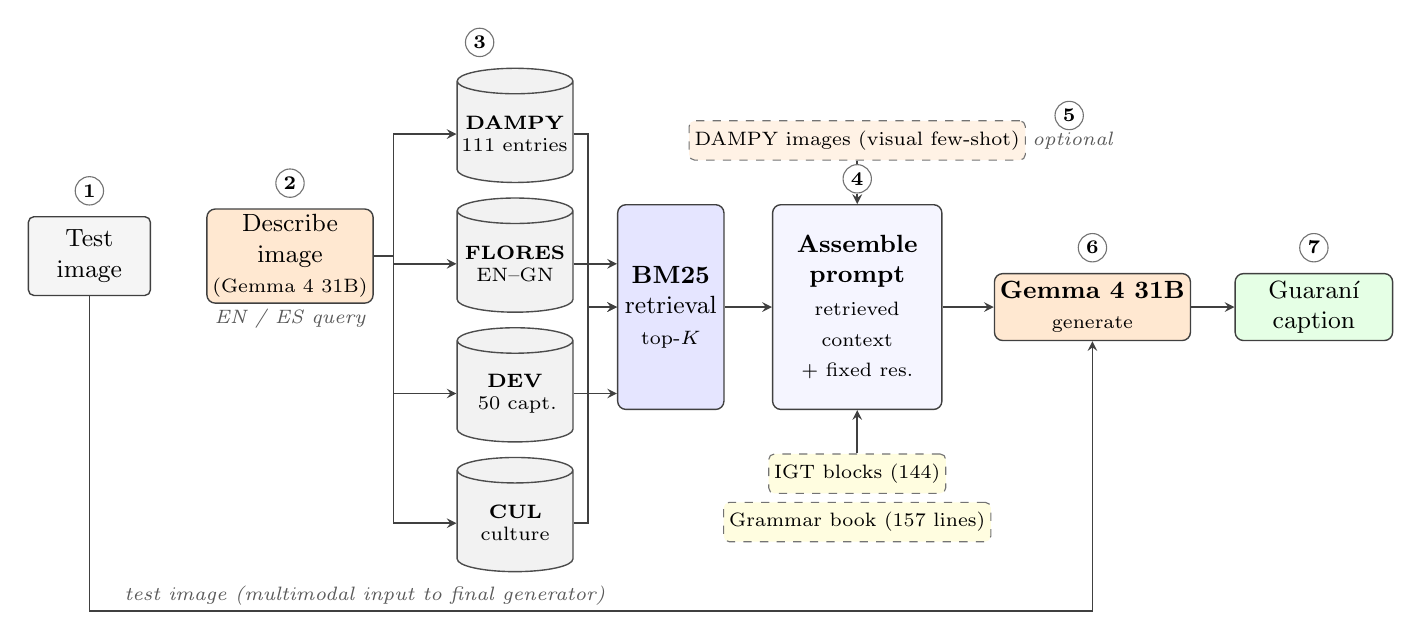
\begin{tikzpicture}[
  font=\small,
  >=stealth,
  node distance=0.55cm and 0.55cm,
  img/.style={rectangle, rounded corners=2pt, draw=black!75, fill=gray!8,
    minimum width=1.55cm, minimum height=1.0cm, align=center,
    line width=0.5pt, inner sep=2pt},
  proc/.style={rectangle, rounded corners=3pt, draw=black!75, fill=blue!7,
    minimum width=1.9cm, minimum height=0.85cm, align=center,
    line width=0.5pt, inner sep=2pt},
  llm/.style={rectangle, rounded corners=3pt, draw=black!75, fill=orange!18,
    minimum width=2.0cm, minimum height=0.85cm, align=center,
    line width=0.5pt, inner sep=2pt},
  pool/.style={cylinder, shape border rotate=90, aspect=0.22, draw=black!70,
    fill=gray!10, minimum height=1.45cm, minimum width=0.85cm, align=center,
    line width=0.5pt, font=\scriptsize, text width=1.4cm, inner sep=1pt},
  fix/.style={rectangle, draw=black!55, fill=yellow!12, dashed, rounded corners=2pt,
    minimum width=2.05cm, minimum height=0.5cm, align=center, font=\scriptsize,
    line width=0.4pt, inner sep=2pt},
  vis/.style={rectangle, draw=black!55, fill=orange!10, dashed, rounded corners=2pt,
    minimum width=2.05cm, minimum height=0.5cm, align=center, font=\scriptsize,
    line width=0.4pt, inner sep=2pt},
  outbox/.style={rectangle, rounded corners=3pt, draw=black!75, fill=green!10,
    minimum width=2.0cm, minimum height=0.85cm, align=center,
    line width=0.5pt, inner sep=2pt},
  ar/.style={->, line width=0.55pt, draw=black!75},
  arD/.style={->, line width=0.55pt, draw=black!75, dashed},
  lab/.style={font=\scriptsize\itshape, text=black!65, inner sep=1pt}
]
% Test image
\node[img] (image) {Test\\image};
% Describe image (Gemma)
\node[llm, right=0.70cm of image] (desc)
  {Describe\\image\\\scriptsize(Gemma 4 31B)};
\node[lab, below=0.02cm of desc] {EN / ES query};
% Four retrieval pools (stacked)
\node[pool, right=1.05cm of desc, yshift=1.55cm] (dampy)  {\textbf{DAMPY}\\111 entries};
\node[pool, below=0.18cm of dampy]                (flores) {\textbf{FLORES}\\EN--GN};
\node[pool, below=0.18cm of flores]               (devp)   {\textbf{DEV}\\50 capt.};
\node[pool, below=0.18cm of devp]                 (cul)    {\textbf{CUL}\\culture};
% BM25
\node[proc, right=0.55cm of flores, yshift=-0.55cm, minimum height=2.6cm,
      minimum width=1.35cm, fill=blue!10] (bm25)
  {\textbf{BM25}\\retrieval\\\scriptsize top-$K$};
% describe -> pools
\draw[ar] (desc.east) -- ++(0.25,0) |- (dampy.west);
\draw[ar] (desc.east) -- ++(0.25,0) |- (flores.west);
\draw[ar] (desc.east) -- ++(0.25,0) |- (devp.west);
\draw[ar] (desc.east) -- ++(0.25,0) |- (cul.west);
% pools -> BM25
\draw[ar] (dampy.east)  -- ++(0.18,0) |- (bm25.west);
\draw[ar] (flores.east) -- (flores.east -| bm25.west);
\draw[ar] (devp.east)   -- (devp.east   -| bm25.west);
\draw[ar] (cul.east)    -- ++(0.18,0) |- (bm25.west);
% Assemble prompt
\node[proc, right=0.6cm of bm25, minimum height=2.6cm, minimum width=2.15cm,
      fill=blue!4] (prompt)
  {\textbf{Assemble}\\\textbf{prompt}\\[1pt]\scriptsize retrieved\\\scriptsize context\\\scriptsize + fixed res.};
\draw[ar] (bm25.east) -- (prompt.west);
% Fixed resources below prompt
\node[fix, below=0.55cm of prompt] (igt)  {IGT blocks (144)};
\node[fix, below=0.10cm of igt]    (gram) {Grammar book (157 lines)};
\draw[ar] (igt.north) -- (prompt.south);
% Optional visual few-shot above prompt
\node[vis, above=0.55cm of prompt] (visdampy)
  {DAMPY images (visual few-shot)};
\draw[arD] (visdampy.south) -- (prompt.north);
\node[lab, right=0.04cm of visdampy] {optional};
% Final generator
\node[llm, right=0.65cm of prompt] (gen)
  {\textbf{Gemma 4 31B}\\\scriptsize generate};
\draw[ar] (prompt.east) -- (gen.west);
% Test image -> generator (multimodal), routed below the diagram
\draw[ar] (image.south) -- ++(0,-4.00) -| (gen.south);
\node[lab] at ($(image.south)+(3.5,-3.80)$)
  {test image (multimodal input to final generator)};
% Output
\node[outbox, right=0.55cm of gen] (cap) {Guaran\'{i}\\caption};
\draw[ar] (gen.east) -- (cap.west);
% Step number badges
\begin{scope}[every node/.style={circle, draw=black!55, fill=white,
    inner sep=0.5pt, font=\scriptsize\bfseries, minimum size=3.6mm}]
  \node at ([yshift=0.32cm]image.north)              {1};
  \node at ([yshift=0.32cm]desc.north)               {2};
  \node[xshift=-0.45cm,yshift=0.32cm] at (dampy.north)        {3};
  \node at ([yshift=0.32cm]prompt.north -| prompt.center)     {4};
  \node[xshift=0.55cm,yshift=0.06cm]  at (visdampy.north east) {5};
  \node at ([yshift=0.32cm]gen.north)                {6};
  \node at ([yshift=0.32cm]cap.north)                {7};
\end{scope}
\end{tikzpicture}
\caption{Overview of the IUHoosiers pipeline for Guaran\'{i} image captioning.
  Given a test image \textbf{(1)}, Gemma~4~31B generates an EN/ES description
  \textbf{(2)} that is used as a BM25 query over four Guaran\'{i} knowledge
  pools \textbf{(3)}: cultural entries (DAMPY), parallel sentences (FLORES),
  dev-set gold captions (DEV), and a curated cultural knowledge base (CUL).
  The retrieved top-$K$ context is combined with fixed resources
  (a 157-line grammar excerpt and 144 interlinear-glossed example blocks)
  into the system prompt \textbf{(4)}. In visual few-shot mode \textbf{(5)},
  DAMPY images with their captions are additionally injected as multimodal
  shots (dashed). Gemma~4~31B \textbf{(6)} consumes the assembled prompt
  together with the test image and produces a Guaran\'{i} caption \textbf{(7)}.}
\label{fig:pipeline}
\end{figure*}

\begin{abstract}
We present IUHoosiers, Indiana University's submission for the
Guaran\'{i} language track in the AmericasNLP 2026 image captioning shared task. Our approach combines large language models with in-context learning
augmented by relevant Guaran\'{i} resources. Specifically, our system
uses Gemma~4 31B together with BM25-based dynamic retrieval from four
Guaran\'{i} knowledge sources (DamPy cultural exemplars, FLORES-200
parallel sentences, dev-set gold captions, and a curated cultural
knowledge base), as well as an optional visual few-shot mode that
injects culturally grounded images as multimodal context.
Across nine submitted configurations, our best system (text BM25,
FLORES $K{=}120$, DAMPY $K{=}15$, CULTURE $K{=}8$) achieves
24.67 chrF++ on the official test set, placing IUHoosiers
first for Guaran\'{i} in human evaluation (3.45/5).
Notably, most of our submitted configurations performed competitively
relative to other participating systems. We also observe a dev-test discrepancy in which visual few-shot retrieval
leads on the 50-image dev set (24.43 vs.\ 23.02 chrF++ for the best text run)
but trails on the 100-image test set (24.04 vs.\ 24.67), underscoring the
limits of small dev-set tuning for visual retrieval.
\end{abstract}

%% ============================================================
\section{Introduction}
%% ============================================================

The AmericasNLP 2026 shared task challenges systems to generate culturally
grounded image captions in indigenous languages of the Americas
\cite{mager-etal-2023-americasnlp}.
We focus on Guaran\'{i}, a tupi-guaraní language that is spoken widely across Paraguay, Brazil, Bolivia, and
Argentina and is the co-official language along with Spanish in Paraguay ($\sim$6.5M speakers). However, it is still considered an under-resourced language across all NLP resources
\cite{chiruzzo-etal-2020-development}.

Cultural captioning for Guaran\'{i} presents two intertwined challenges.
First, captions must be \textit{culturally accurate}: correctly distinguishing
closely related cultural items, such as \textit{mat\'{e}} from its cold counterpart
\textit{terer\'{e}}, requires culturally grounded knowledge that generic
vision-language models often lack.
Second, captions must be \textit{linguistically reflective} as Guaran\'{i} is
agglutinative with active/inactive voice morphology and pervasive Spanish
borrowing in everyday \textit{jopara} speech \cite{estigarribia2020}.

Since the dev set contains only 50 image-caption pairs and the gold labels
follow a specific format, parameter-efficient fine-tuning methods
such as PEFT \cite{peft} and LoRA \cite{hu2022lora} may be prone to
overfitting without substantial data augmentation. We therefore focus on
inference-time methods instead.
Recent work suggests that grammar-book and parallel-text context can
improve low-resource language generation without gradient updates
\cite{tanzer2023,aycock2024,zhang2025}, and we build on this finding with
\textbf{retrieval-augmented prompting}.
For each test image, we generate a text description, query four Guaran\'{i}
knowledge pools with BM25 \cite{robertson2009bm25}, and inject the top-$K$
retrieved items into the system prompt of Gemma~4 31B \cite{gemma4_2025}
to generate captions in a single forward pass.
Additionally, we explore a \textit{visual few-shot} mode that injects cultural images from Diccionario audiovisual multilingüe del Paraguay (DAMPY)\footnote{\url{https://spl.gov.py/dampy/index.html}} as multimodal context.
Figure~\ref{fig:pipeline} gives an overview of the full pipeline.

\begin{comment}
Our main contributions are:
\begin{itemize}
  \item A retrieval-augmented multimodal system for Guaran\'{i} image
    captioning requiring no fine-tuning and using four complementary
    Guaran\'{i} knowledge pools.
\footnote{Code is available at \url{https://github.com/victorshi119/Cultural_Image_Captions_2026}}
  \item An empirical analysis across IUHoosiers' nine submissions revealing a systematic
    dev--test discrepancy between text BM25 and visual few-shot retrieval.
  \item Parameter ablation study helps us locate the idea retrieval depth for the highest performing result: moderate FLORES expansion (K=120) and a broadened cultural knowledge pool (K=8) yield the
    best test-set chrF++.
\end{itemize}
\end{comment}

%% ============================================================
\section{System}
%% ============================================================

\paragraph{Why in-context learning?}
The AmericasNLP 2026 shared task spans five indigenous languages (Guaran\'{i},
Bribri, Yucatec Maya, Wix\'{a}rika, and Nahuatl), each with very distinct
typological properties, morphological systems, and cultural contexts. We
believe the linguistic and cultural distances among these languages are too
vast for any single unified system to address all of them effectively, and we
take the view that in low-resource settings, building one dedicated system per
language is the more principled approach. A language-specific pipeline allows
much more targeted injection of relevant grammatical structure and cultural
knowledge than a one-size-fits-all system could provide.
We therefore build a Guaran\'{i}-specific pipeline and adopt in-context
learning (ICL) as our core method. Recent work on extremely low-resource
languages shows that ICL, especially when paired with explicit linguistic signals, can outperform parameter-efficient fine-tuning when the target language is poorly represented in the base model
\citep{li-etal-2025-context-learning}. At the same time, work on culturally aware vision-language modeling has shown that standard VLMs often miss
fine-grained cultural distinctions, and that improving cultural grounding may
require either specialized data construction or model adaptation
\citep{huang2025cultureclip}. Our approach therefore tests whether carefully
selected grammatical and cultural knowledge, injected at inference time, can
close this gap without any parameter updates.%, and we aim to provide a reproducible baseline for future work that may combine ICL, retrieval, and fine-tuning once larger Guaran\'{i} image--caption datasets become available.

\paragraph{Model.}
We use Gemma~4 31B \cite{gemma4_2025}, a 31-billion-parameter
vision-language model with a 128K-token multimodal context window, which is accessed via the IU ReaLLMs API\footnote{\url{reallms.rescloud.iu.edu}}, an OpenAI-compatible endpoint
hosted by Indiana University Research Technologies on the BigRed~200
HPC cluster.
The original baseline prompt (Spanish-language Guaran\'{i} captioning guidelines)
is used for all nine submissions.\footnote{Code is available at \url{https://github.com/victorshi119/Cultural_Image_Captions_2026}}

\paragraph{Fixed resources.}
Two resources are injected into every prompt regardless of the test image:
a 157-line grammar-book excerpt from \citet{estigarribia2020grammar} covering
Guaran\'{i} morphosyntax, voice alternations, and postpositional structure,
and 144 interlinear glossed example blocks
(surface form / morpheme break / gloss / translation). 
These were selected on the basis of a prior 64-subset ablation over six
grammar resource types (Grambank features, FLORES parallel pairs, interlinear
glosses, grammar-book parallel sentences, grammar-book prose, and an
Apertium morphological reference). 

We note that these distilled resources were generated with the assistance
of Claude in a two-step process. First, we provided Claude with the raw
resource files together with the competition setting and asked it to reason
about the most effective format for injecting such resources into a language
model for in-context learning. Through iterative discussion, Claude then
produced prompts designed to reorganize and condense the original materials
into more model-friendly representations. In a second, separate session, we
supplied Claude with the raw text resources together with the generated
prompt in order to produce the final distilled resources. Additional details
are provided in the Appendix.
%The ablation showed grammar-book prose and parallel examples to be the most consistently helpful static resources \cite{aycock2024}. It's important to also note that FLORES pairs hurt when injected statically, motivating the switch to BM25-retrieved FLORES in the final system.

\paragraph{Dynamically retrieved pools.}
For each test image a text description is generated and used as the BM25 query \cite{robertson2009bm25}.
Four resource pools are indexed and queried per image:
\begin{enumerate}
\item \textbf{DAMPY}: 111 culturally grounded entries from DamPy,
Paraguay's official audiovisual dictionary (42 food, 47 fauna, and 22 flora entries),
each with bilingual Spanish/Guaran\'{i} labels. We note that the DamPy dataset we
scraped from the internet does not provide captions. Therefore, we asked a frontier
model (Claude) to generate bilingual captions for the dataset.
\item \textbf{FLORES}: EN$\to$GN parallel sentence pairs from FLORES-200
    \cite{nllb-team-2022-scaling}, providing in-domain Guaran\'{i}
    sentence structure across a broad topical distribution.
\item \textbf{DEV}: the 50 gold Guaran\'{i} dev-set captions, retrieved
by BM25 text matching per image, providing an in-domain captioning style.
We further augmented the dataset with parallel English--Guaran\'{i} captions by
asking Claude to generate the English captions, since the competition
only provides Guaran\'{i} labels. These English captions help us retrieve
relevant images later during the RAG step.
\item \textbf{CUL}: a curated Guaran\'{i} cultural knowledge base
    consisting of text chunks describing food, crafts, and cultural
    practices. Since the CUL file is relatively small, it is always
    injected into the system prompt regardless of the retrieval setting.
    We hypothesize that adding retrieved CUL examples can further help
    reinforce culturally relevant concepts appearing in the image.
    \end{enumerate}

To be specific, the retrieval works as follows: we first build a BM25 index over either grammar sections for CUL, which is organized by section, or paired entries for DAMPY, FLORES, and DEV. Then, depending on the dataset, we ask a language model (Gemma 4 31B) to first describe the image in the relevant language, using English for FLORES and Spanish for DAMPY, CUL, and DEV. We then use BM25 to retrieve the corresponding relevant Guaran\'{i} examples.

For visual few-shot runs, instead of injecting only retrieved text examples, we retrieve the top-$K$ DAMPY entries using BM25 over Spanish image descriptions generated by the language model. The corresponding images and Guaran\'{i} captions are then injected as multimodal few-shot examples in the prompt.

%For visual few-shot runs, instead of doing text retrieval on the generated caption for DAMPY, we employ an image-embedding similarity search: the top-$K$ most visually similar DAMPY images are injected as multimodal few-shot turns in the prompt.

\paragraph{Prompt structure.}
Each request follows a four step process:
\begin{enumerate}
    \item \textbf{System prompt:}
    Contains the captioning guidelines, fixed grammar resources,
    and dynamically retrieved context blocks from CUL, DAMPY,
    FLORES, and the dev captions.

    \item \textbf{Multimodal few shot prompting:}
    Optional multimodal few shot examples are injected depending
    on the retrieval setting. For visual few shot runs, the
    retrieved DAMPY image caption pairs are inserted here as
    multimodal demonstrations.

    \item \textbf{Test image:}
    The query image is provided to the model.

    \item \textbf{Generation:}
    The model generates a caption in Guaran\'{i}.
\end{enumerate}
%\paragraph{Prompt structure.}
%Each request follows a fixed four-part structure:
%(1)~\textbf{System prompt}, containing captioning guidelines, fixed grammar
%resources (all lines in the distilled grammar book and IGT), and the dynamically retrieved context blocks (CUL, DAMPY, FLORES,
%dev captions) in that order;
%(2)~\textbf{Five fixed few-shot turns}, pairing dev images with their
%gold Guaran\'{i} captions;
%(3)~\textbf{Test turn}, the query image;
%(4)~\textbf{Generation}, caption output in Guaran\'{i}.
%For visual few-shot runs, the visual DAMPY shots are injected as multimodal
%turns immediately before the five fixed few-shot pairs.

\paragraph{Configurations.}
Table~\ref{tab:configs} lists all nine submissions.
Runs v0-v7 use text-based retrieval across all four pools, with RAG
selecting top-$K$ examples except for v6, which uses static selection
from DAMPY.
Run v8 replaces DAMPY text examples with visual shots, using static
selection of the first 10 images from the dataset.
\begin{table}[t]
\centering
\small
\setlength{\tabcolsep}{3pt}
\begin{tabular}{clrrrr}
\toprule
\textbf{Ver} & \textbf{Mode} & \textbf{DMP} & \textbf{FLR} & \textbf{DEV} & \textbf{CUL} \\
\midrule
v0 & text+RAG   &  5 & 100 &  5 &  5 \\
v1 & text+RAG   & 10 & 100 & 10 &  5 \\
v2 & text+RAG   & 15 & 100 & 10 &  5 \\
v3 & text+RAG   & 20 & 100 & 10 &  6 \\
v4 & text+RAG   & 15 & 120 & 10 &  8 \\
v5 & text+RAG   & 15 & 150 & 10 & 10 \\
v6 & text+static & 3 & 30 & 0 & 0 \\
v7 & text+RAG   & 10 & 100 & 10 &  5 \\
\midrule
v8 & visual+static & 10 & 30 & 0 & 0 \\
\bottomrule
\end{tabular}
\caption{Nine submission configurations.
  \textbf{DMP}: DAMPY shots. \textbf{FLR}: FLORES shots.
  \textbf{DEV}: dev-set shots. \textbf{CUL}: cultural knowledge shots.
  In \textbf{RAG} mode, shots are selected by retrieval score; in
  \textbf{static} mode, the first $n$ examples from the dataset are used.
  All runs include grammar book (157 lines) and interlinear (144 blocks)
  as fixed context.}  \label{tab:configs}
\end{table}

%% ============================================================
\section{Results}
\subsection{Dev-set Results}
Table~\ref{tab:devresult} shows the results for each configuration on the dev set. We note that since we are evaluating against the dev set, the DEV few-shot examples were not used.

\begin{table}[t]
\centering
\small
\setlength{\tabcolsep}{3pt}
\begin{tabular}{clr}
\toprule
\textbf{Ver} & \textbf{Mode} & \textbf{chrF++} \\
\midrule
v0 & text+RAG    & 22.40 \\
v1 & text+RAG    & 22.02 \\
v2 & text+RAG    & 21.59 \\
v3 & text+RAG    & 21.90 \\
v4 & text+RAG    & 21.44 \\
v5 & text+RAG    & 20.43 \\
v6 & text+static & 22.49 \\
v7 & text+RAG    & 22.02 \\
\midrule
v8 & visual+static & 24.17 \\
\bottomrule
\end{tabular}
\caption{Nine submission configurations and their dev-set chrF++ scores.}
\label{tab:devresult}
\end{table}

%% ============================================================

\subsection{Test-Set Results}

Table~\ref{tab:results} shows official test-set chrF++ and CIDEr for
all IUHoosiers submissions alongside competing teams.
The best submission (v4) achieves 24.67 chrF++ and 0.149 CIDEr,
a 4.53-point gain over the official baseline (20.14) and a 1.57-point margin
over the next-best team (gators, 23.10).
IUHoosiers placed first for Guaran\'{i} in human evaluation with a
mean annotator rating of 3.45/5, versus 3.30 for the second-ranked
team; eight of our nine submissions outscore every other team's best result.

\begin{table}[t]
\centering
\small
\setlength{\tabcolsep}{4pt}
\begin{tabular}{llrr}
\toprule
\textbf{Team} & \textbf{Ver} & \textbf{chrF++} & \textbf{CIDEr} \\
\midrule
IUHoosiers & v4 & \textbf{24.67} & 0.149 \\
IUHoosiers & v5 & 24.42 & \textbf{0.167} \\
IUHoosiers & v1 & 24.41 & 0.135 \\
IUHoosiers & v8 & 24.41 & 0.135 \\
IUHoosiers & v2 & 24.41 & 0.143 \\
IUHoosiers & v0 & 24.39 & 0.124 \\
IUHoosiers & v3 & 24.16 & 0.128 \\
IUHoosiers & v6 & 24.04 & 0.112 \\
IUHoosiers & v7 & 22.43 & 0.074 \\
\midrule
gators      & v0 & 23.10 & 0.124 \\
baseline    & v0 & 20.14 & 0.005 \\
Mila        & v1 & 19.77 & 0.031 \\
usp         & v0 & 19.73 & 0.024 \\
NAIST       & v0 & 19.41 & 0.046 \\
\bottomrule
\end{tabular}
\caption{Official test-set leaderboard (selected entries).
  Eight of nine IUHoosiers submissions outperformed all other teams.
  v5 achieved the highest CIDEr despite not having the best chrF++.}
\label{tab:results}
\end{table}

%Notably, v4 led on chrF++ (24.67) while v5 led on CIDEr (0.167).
%CIDEr uses TF-IDF weighting that rewards the successfully detection of Guaran\'{i} vocabulary.
%v5's larger FLORES context (K=150) and broader cultural pool (K=10) were able to expose the model to greater lexical variety, which led it to be able to produce semantically precise captions that score well under CIDEr but have slightly lower character-level
%overlap with the reference.
%This metric divergence appears to suggest that no single automatic metric fully captures caption quality in our case, and the human evaluation, a more convincingly and time-costly metric, confirmed the overall great performance of our model.

\begin{comment}
\subsection{Dev-Set Calibration}

Table~\ref{tab:dev_results} shows chrF++ on the 50-image dev set from our
calibration experiments.
These experiments used \textit{static injection} (fixed FLORES sentence
counts and DAMPY category counts), a different parameter space from the final
test submissions which use BM25 dynamic retrieval; the two config spaces
cannot be mapped 1:1.

\begin{table}[t]
\centering
\small
\setlength{\tabcolsep}{5pt}
\begin{tabular}{llr}
\toprule
\textbf{Mode} & \textbf{Config (FLR / DMP)} & \textbf{chrF++} \\
\midrule
visual & 15 shots / FLR=50 & \textbf{24.43} \\
visual & 10 shots / FLR=30 & 24.17 \\
visual &  5 shots / FLR=30 & 23.49 \\
\midrule
text   & FLR=100, DMP=5    & \textbf{23.02} \\
text   & FLR= 30, DMP=3    & 22.49 \\
text   & FLR= 80, DMP=3    & 22.21 \\
text   & FLR= 50, DMP=5    & 22.09 \\
text   & FLR= 20, DMP=2    & 21.80 \\
text   & FLR= 50, DMP=3    & 21.43 \\
\bottomrule
\end{tabular}
\caption{Dev-set calibration results (static injection, 50 images).
  \textbf{FLR}: FLORES sentences injected.
  \textbf{DMP}: DAMPY caption categories injected.
  For visual runs, DAMPY images are injected as few-shot context.
  Dev and test submissions use different parameter spaces.}
\label{tab:dev_results}
\end{table}

Visual few-shot consistently outperformed text injection on the dev set across
all shot counts.
The best visual configuration (15 shots, FLR=50) was able to achieve 24.43 chrF++, which is a
1.41-point lead over the best text configuration (FLR=100, DMP=5: 23.02).
Among text runs, more FLORES context is not uniformly better on dev. As seen from the table,
the FLR=30 run (22.49) beats FLR=50 and FLR=80, with improvement only at
FLR=100.
These calibration findings motivated our decision to submit nine test configurations
covering both strategies and a wide FLORES depth sweep.
\end{comment}

%% ============================================================
\section{Analysis}
%% ============================================================

\begin{comment}
    
\subsection{Dev--Test Discrepancy}

Visual runs dominated the dev set (24.43 chrF++ for the 15-shot static
configuration) but underperformed using text BM25 on the test set (24.04 for v6).
On the test set, text BM25 v4 achieved 24.67 chrF++ while the best visual run (v6,
15 shots) only reached 24.04 chrF++, which is a 0.63-point swing in favor of text that
reverses the 1.41-point visual lead observed on dev.

We suspect that this observation could be due to three factors.
First, the 50-image dev set is small and partially overlaps with the
five fixed few-shot images; visual retrieval is more sensitive to this
instability because visual similarity retrieval is more likely to return
an exemplary image that the model has already seen in its few-shot context.
Second, the 100-image test set covers a wider cultural distribution, and
the 111-entry DAMPY pool lacks visual exemplars for many test categories as it only covers food, flora and fauna. With that being said, when no relevant visual exemplar exists, visual retrieval could return misleading information.
Third, broader FLORES context (K=120/150) could have generalized across diverse
test-image topics in a way that visual retrieval cannot when the relevant exemplar is absent.
\end{comment}
\begin{comment}
\subsection{Retrieval Depth}

Among text BM25 runs, the optimal configuration (v4) is neither the smallest nor the largest context window, which indicated that it is in the best configuration setting for retrieval depth.

%\paragraph{FLORES depth.}
Increasing FLORES from K=100 (v0--v3: 24.16--24.41) to K=120 (v4: 24.67)
yields a 0.26--0.51-point gain in test chrF++.
Further increasing to K=150 (v5: 24.42) slightly drops chrF++, which could suggest that the worsening of the model performance likely occurs once the most relevant FLORES pairs are
already retrieved.

\paragraph{DAMPY depth.}
The DAMPY pool works best at K=15 (v2, v4, v5).
Reducing to K=5 (v0: 24.39) led to slightly worse results whie increasing to K=20 (v3: 24.16) substantially hurt, which suggests that
retrieving too many DAMPY captions dilutes the prompt with
low-relevance cultural exemplars.

\paragraph{Visual shots.}
Among visual runs, 50 shots (v8: 24.41) substantially outperform
15 shots (v6: 24.04) and 25 shots (v7: 22.43).
The non-monotonic dip at 25 shots may reflect a retrieval alignment issue
in that specific run.
At 50 shots, v8 matches the test chrF++ of the mid-range text BM25 runs
(v1, v2) exactly (24.41), which helped confirm that visual few-shot can close the
gap with text BM25 but requires high shot counts to stabilize.
\end{comment}
\subsection{Qualitative Analysis}

\paragraph{Submission selection.}
We selected these nine configurations from a larger candidate pool, with final choices informed by chrF++ scores alongside our personal judgement and our team's working knowledge in Guaraní and Jopara. While chrF++ was a useful signal for tracking progress during the pilot phase, final selection was not driven by it alone, as the metric measures character n-gram overlap against a single gold reference and is therefore blind to semantic paraphrase and cultural correctness. A caption that correctly identifies a
cultural item but uses different surface forms than the reference can score no
better than one that gets the cultural content wrong while sharing incidental
n-grams.
Instead, selection applied two criteria.
First, \textit{output style}: captions should match the concise, visually
specific register of the dev-set gold labels and avoid formulaic boilerplate
appended regardless of image content.
Second, \textit{cultural accuracy}: captions should correctly identify
culturally specific items, especially when the discriminating cue is visual and subtle.
The BM25 retrieval pipeline supports both: FLORES parallel context shapes linguistic register and fluency, while DAMPY retrieval and the five fixed few-shot exemplars anchor culturally grounded vocabulary.

One notably culturally specific image among the first ten test examples is \textbf{grn\_052}, depicting a mat'{e} setup (gourd, bombilla, \textit{pava} kettle). All text BM25 configurations incorrectly label it \textit{terer\'{e}},
the more frequently mentioned drink in the FLORES and DAMPY corpora.
The 15-shot visual run (v6) correctly identifies it as mat\'{e} by
retrieving a visually similar dev exemplar. The discriminating cue, the
metal \textit{pava} rather than a cold thermos, is a visual signal
unavailable to text retrieval. Visual retrieval therefore gains cultural
precision at the cost of lower surface n-gram overlap when its retrieved
vocabulary diverges from the reference phrasing.

Text runs also tend to add repeated generic closing phrases
(e.g., \textit{``Ko tembi'u ha'e peteĩ rembiapokue tee Paraguáigui''},
``this dish is a true cultural product of Paraguay'') regardless of image
content, while gold captions use more varied, image-specific language.
The visual runs produce more image-specific descriptions, which explains
their higher qualitative character despite lower chrF++ on the test set.
The human evaluation's preference for IUHoosiers (3.45/5) over competitors
reflects the generally higher Guaran\'{i} output quality compared to
translation-based baselines.

%% ============================================================
\section{Conclusion}
%% ============================================================
IUHoosiers achieved first place for Guaraní at AmericasNLP 2026 using Gemma 4 31B with BM25-augmented retrieval from four Guaraní knowledge sources. Beyond the result itself, the most practically useful contribution is the pipeline design: language-specific knowledge injection at inference time without fine-tuning rather than any particular hyperparameter choice. The broader takeaway is that carefully curated grammar and cultural resources, injected at inference time, can remain competitive without parameter updates. That is the durable result worth carrying forward.
%The key practical finding is that text BM25 with moderate FLORES expansion (K=120) and a broadened cultural knowledge pool (K=8) wins on test-set chrF++, while the 50-shot visual configuration closes most of this gap. Dev-set rankings are unreliable predictors of test-set rankings; visual few-shot led dev by 1.41 points while lagging test by 0.63 points, a reversal attributable to the dev set's small size and partial contamination. Future work should explore adaptive retrieval that selects modality per image based on retrieval confidence, larger DAMPY visual pools, and fine-tuning once a larger set of culturally grounded Guaran\'{i} images with consistent and reliable captions are available.

%% ============================================================
\section*{Acknowledgments}
%% ============================================================

We thank Indiana University Research Technologies for ReaLLMs API
access and the BigRed~200 HPC cluster, and the AmericasNLP 2026
organizers for the dataset and evaluation infrastructure.

%% ============================================================
\bibliography{custom}

\end{document}